\chapter{Experimental Evaluation} \label{chap6}

In this chapter, we design and conduct the experiments to support
the validation of our approach, WfSteer, to address the problem 
and hence the validation of this thesis's hypothesis.
Our hypothesis encompasses WfSteer's instantiation both for workflow scripts and for WMS, and within each instantiation we further distinguished between allowing for tracking steering actions and keeping the execution overhead low. This chapter follows this separation. 
Section \ref{sec_exps_wfscripts} presents the validation of WfSteer for workflow scripts, showing a qualitative analysis on allowing for tracking steering actions and a quantitative evaluation on the execution overhead, using real-world use cases in the O\&G industry. Analogously, Section \ref{exps_wms} has the validation of WfSteer's instantiation into a WMS, following this same organization.

\section{Managing Steering Action Data in Workflow Scripts}
\label{sec_exps_wfscripts}

In this section, we present the experiments to aid the validation of one of the instantiations of WfSteer,
DfAdapter, in a real-world workflow script, libMesh-sedimentation.
DfAdapter has been introduced in Chapter \ref{chap_dfadapter} and libMesh-sedimentation has been briefly introduced in Section \ref{sub_libmesh}.
We show how users can monitor and understand, at runtime, the impact of their steering actions by relating steering action data with
provenance, domain, and execution data, then we evaluate the added overhead in a workflow script.
We begin by providing implementation details of how DfAdapter is coupled with libMesh-sedimentation (Sec. \ref{subsec_libmesh_exp_use_case}),
afterwards we present steering action data analysis in libMesh-sedimentation workflow (Sec. \ref{sec_steering_action_analysis_workflow_script}), and
conclude with an overhead evaluation (Sec. \ref{sec_overhead_eval_wokflow_script}).



\subsection{Use case: Computational Fluid Dynamics in Geoscience with libMesh-sedimentation}
\label{subsec_libmesh_exp_use_case}

libMesh-sedimentation provides a real and rich case for parameter tuning for the following reasons. First, it is a CSE application that requires HPC to run a simulation with over 70 parameters, which may be modified by the user for better performance and accuracy of results \cite{Camata2018In}. Second, as this simulation may last for weeks, the user does several tunings and there is no tracking for them. Third, there is a strong potential for richer online data analyses with steering action data by correlating the steering data to domain-specific values (mainly QoIs) and other data in the workflow database.

To use DfAdapter in libMesh-sedimentation, we follow the utilization guide described in Section \ref{dfadapter_utilization}.
The first step is modeling libMesh-sedimentation simulation as a workflow and identifying analysis and adaptation points. Workflow data are captured by DfAnalyzer. Application-specific data are modeled as new tables of the relational database schema for the workflow database (Fig. \ref{fig:dfadapter_wfdbschema}).
The main input dataset that the user adapts is the input for the loop evaluation data transformation, named \codefont{I\_Iteration\_Params}, which contains input parameters for the numerical solvers. The users specify parameters in a setup configuration file. The workflow script checks, at every time step, if any modification has been made to this file. If a modification occurred, the parameters are redefined according to the new values. That is, libMesh-sedimentation implements a file-based checks approach for the adapter service (Sec. \ref{wfscript_system-design-principles}).
Modifications in this file happen within an implementation of the Adapter API. The implementation receives parameters and new values and modifies the file according to the inputs.
 The last step is to insert steering action data capture API calls in the adaptation points.
 In libMesh-sedimentation code, it is inserted immediately after the parameters are reloaded when there is a modification in the configuration file.
 Finally, when the user steers, DfAdapter captures provenance, domain and steering action data every time it detects user steering actions.
 Figure~\ref{fig:libmesh_sed_cppode} 
 shows the instrumentation
 of libMesh-sedimentation with workflow data capture calls (using DfAnalyzer's API --- Sec. \ref{dfadapter-implementation-details}) and steering action data capture calls.


\begin{figure}[H]
    \centering
    \includegraphics[width=\textwidth,keepaspectratio]{img/libmesh-experiment.pdf}
    \caption{libMesh-sedimentation workflow script code with added API calls along with its  workflow representation.}
    \label{fig:libmesh_sed_cppode}
\end{figure}



\textbf{HPC Environment and Deployment}. The experiments in this section were conducted on Lobo Carneirno cluster\footnote{http://www.nacad.ufrj.br/recursos/sgiicex}, an SGI ICE X with 252 nodes, each with a 24-core processor and 64 GB RAM, summing 6,048 cores and 16 TB RAM. The nodes are interconnected via FDR InfiniBand and share a Lustre file system with 500 TB. The Data Management services and MonetDB are deployed on a separate node in the cluster, different from the ones used by the main computational process for libMesh-sedimentation.
libMesh-sedimentation is implemented in C++ and its code with instrumentation for analysis and steering is available on GitHub \cite{libMeshSed_github} along with with DfAdapter's code \cite{DfAdapterGitHubDfAdapter}.





%%%%%%%%%%%%%%%%%%%%%%%%%%%%%%%%%%%%%%%%%%%%%%%%%%%%%%%
%%%%%%%%%%%%%%%%%%%%%%%%%%%%%%%%%%%%%%%%%%%%%%%%%%%%%%%
%%%%%%%%%%%%%%%%%%%%%%%%%%%%%%%%%%%%%%%%%%%%%%%%%%%%%%%
%%%%%%%%%%%%%%%%%%%%%%%%%%%%%%%%%%%%%%%%%%%%%%%%%%%%%%%
%%%%%%%%%%%%%%%%%%%%%%%%%%%%%%%%%%%%%%%%%%%%%%%%%%%%%%%





\subsection{User Steering Action Data Analysis}
\label{sec_steering_action_analysis_workflow_script}

\subsubsection{Small-scale case}
\label{sub_dfadapter_experiments}


The small-scale experiment is used by scientists as a benchmark to
evaluate sedimentation solvers. It simulates the laboratory test carried
out by \citet{DeRooij2001Time-} with a
lock-exchange configuration. The objective of this experiment is to show
the data analytical potential of our solution, how we record structured
parameter-tunings, and how users can query the steering action data to
enhance their analyses.

The computational setup used in this test case consists of a plane
channel with dimensions $20 * 2$ filled with sediments in suspension and
clear fluid at rest. In the laboratory, a lock-gate is used to separate
the fluids before the beginning of the experiment. When the gate is
removed, a mutual intrusion flow develops in which the particle-laden
front travels along the bottom to the right. In this simulation, the
lock-gate is located at $x = 0.75$. The non-dimensional parameters used
are $Grashof \text{ } number = \num{5.0e-6}$, $Schmidt \ number = 1.0$,
and $Settling \text{ } velocity = 0.02$. Adaptive mesh refinement is used to track
the interface between sediments concentration and clear water. Figure \ref{fig:2dtanks}
shows the concentration of sediments in suspension and the adapted mesh
at simulation time $t = 10$.

\begin{figure}[H]
    \centering
    \includegraphics[width=\textwidth,keepaspectratio]{img/tank2d.pdf}
    \caption{2D visualization of the tank and the concentration of sediments. This figure was generated at simulation time $t = 10$.}
    \label{fig:2dtanks}
\end{figure}

In this simulation, the user is interested in analyzing possible performance gains when the number of nonlinear and linear (in this case, GMRES) iterations is tuned at runtime. Specific fine-tunings on different input parameters may impact the solvers and hence the simulation time considerably. During the execution, the user submits analytical queries. Based on the analyses of nonlinear and GMRES iterations, the user decides to fine-tune the solver’s parameters. In total, the user chooses to do six fine-tunings in 10 hours of simulation. Figure \ref{fig:q1steering} shows a query
that tracks the steering action. The query lists the parameters tuned by a user (say, Bob), correlated to the time steps. By running this query, other researchers are aware that Bob adapted this workflow execution six times. The times and values are well-structured and recorded in the workflow database.

\begin{figure}[H]
    \centering
    \includegraphics[width=\textwidth,keepaspectratio]{img/param_tun_q1.pdf}
    \caption{Query analyzing the track of the steering actions.}
    \label{fig:q1steering}
\end{figure}


Figure \ref{fig:q2steering} shows the query results
of the average values of strategic quantities ten iterations before and after each of the  fine-tunings. The results include nonlinear and linear (GMRES)
iterations, which are output values of the solver, and the number of
finite elements, which is an output of the mesh refinement process and
depends on other inputs of the solver. This query shows an integration
of provenance, domain, and execution data, and the new steering action data we introduced.

\begin{figure}[H]
    \centering
    \includegraphics[width=\textwidth,keepaspectratio]{img/param_tun_q2.pdf}
    \caption{Query integrating execution, domain, provenance, and steering action data.}
    \label{fig:q2steering}
\end{figure}

The results in Figure \ref{fig:q2steering} (we highlight the main findings)
show that the Tunes \#3, \#4, and \#6 impacted the average elapsed time
and the average number of GMRES iterations, which are of high interest
to the user. Tune \#5 barely changed the other values but reduced the
number of mesh elements by about 11.15\%. This reduction is important
because when there are too many elements, out-of-memory errors may
happen (see the large-scale case next). In Figure \ref{fig:sixtunings}, we plot the evolution of
these variables over time and annotate the tunings (Tune \#1 to Tune
\#6) so the user can evaluate the adaptations.


\begin{figure}
    \centering
    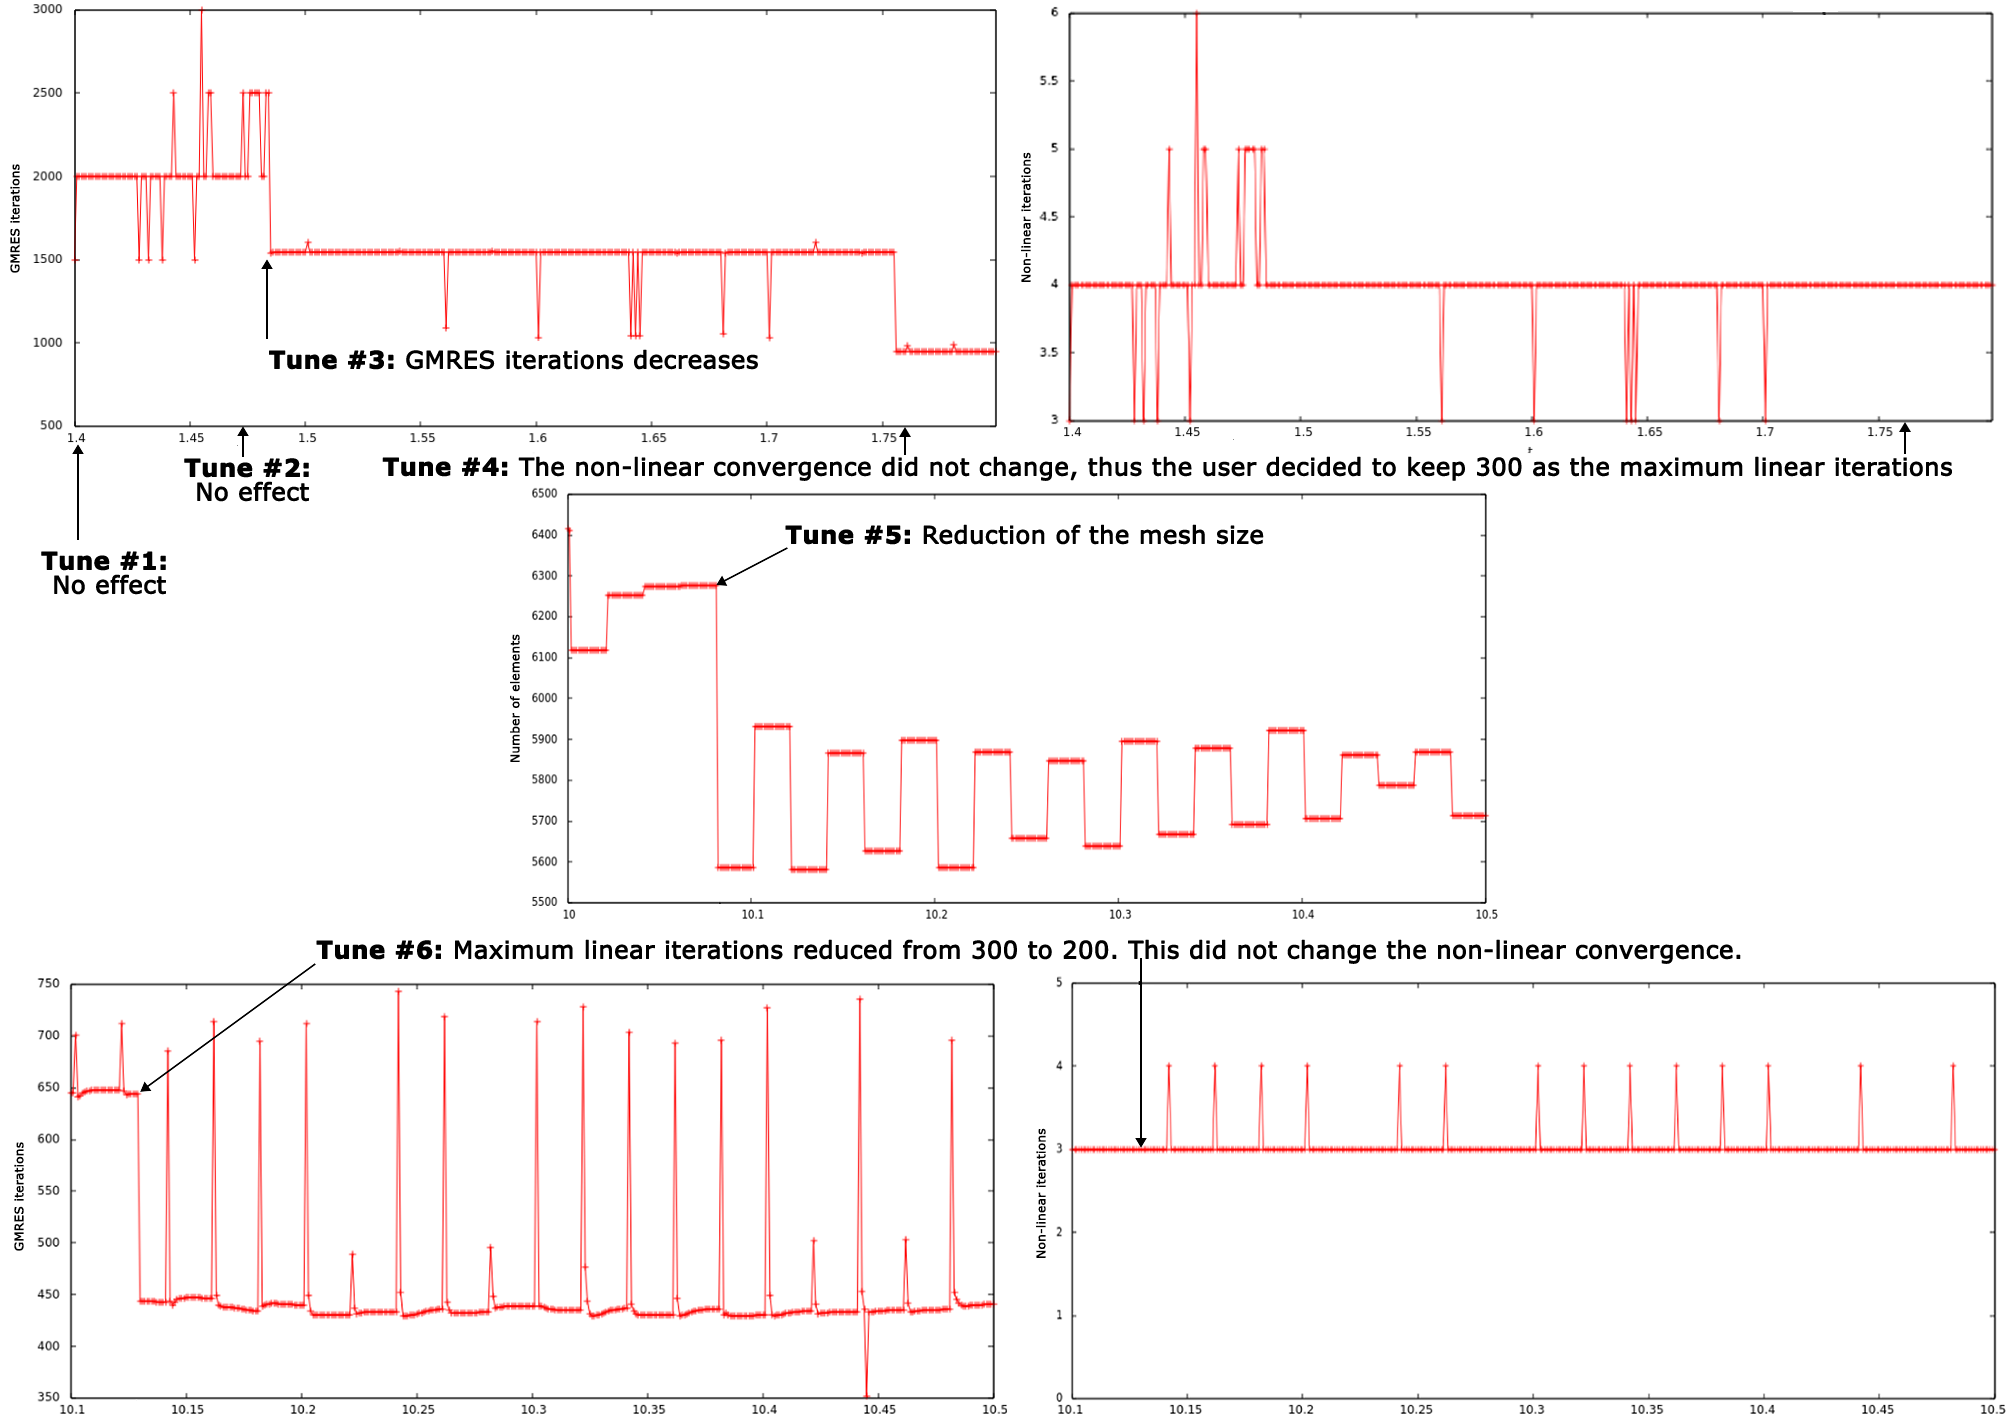
\includegraphics[width=\textwidth,keepaspectratio]{img/tunes-1-to-6.png}
    \caption{Plots of monitoring queries for number of GMRES iterations, non-linear iterations, and mesh elements over time. We highlight the tune actions.}
    \label{fig:sixtunings}
\end{figure}


Based on the online analyses of user steering action data, the user
 decides whether new tunes are needed. Moreover, considering a scenario where another research team
analyzes the provenance of the results, the team sees the abrupt changes in
the results and can correlate these results with Bob's steering actions
through SQL queries in the workflow database. They can check if sudden
changes are related to one of the adaptations Bob did. Thus, they will
have a better understanding of the results.

\subsubsection{Large-scale case}

In a large-scale experiment, \crossref{A4: faltou descrever qtos nós do LoboC foram usados} using 480 cores of Lobo Carneiro cluster, the user sets up the libMesh-sedimentation
workflow with a simulation of the deposition of sediments carried by a
turbidity current over a real experimental channel. A mixture of
sediments is continuously injected into a channel that deposits
sediments in the tank. The tank has $length = 135$, $width = 40$, and $height
= 50$ (dimensionless units).

The dimensionless simulation parameters are $Settling \text{ }  velocity =
\num{5.36e-6}$, $Grashof \text{ }  number =
\num{3.42e7}$, $Schmidt \text{ }  number = 1.0$, and fixed $time \text{ }  step =
0.01$.
It uses a 3D simulation with a spatial discretization using an
initial unstructured mesh with 1.2 million tetrahedra. AMR/C is employed
and three levels of uniform refinement are applied before the time loop.
The user specifies input parameter values for the sedimentation solver
(\ie{} linear and non-linear tolerances, the maximum number of linear
iterations, tolerances for AMR/C error estimation and refinement and
coarsening fractions) aiming at attaining a high-fidelity simulation.
One strategic simulation data that quantifies such level of detail is
the number of elements obtained in the mesh refinement data
transformation (the second one in the time loop). Although a large number of
elements in the mesh means a high level of detail, it also means more
memory and time consumed by the simulation. Depending on the parameter
values specified for the solver, the simulation may run out of memory.
Thus, the user does not know beforehand which range of parameters is
best for a good level of detail with acceptable memory consumption.

To support the user in following the evolution of strategic values, we
use our monitoring approach by setting up queries to the workflow database at specified time intervals (each simulation's time step). One query shows
linear and nonlinear iterations, residual norms, and the number of
elements in the mesh at each time step. Additionally, ParaView Catalyst
is set up to plot 3D visualizations of the channel and the sediment
deposits over time. Then, the user sees, for example, that the number of
elements generated by the AMR/C is close to a maximum preset number of
elements. At that rate, the simulation may crash, running out of memory.
The user knows that by changing some of the solver parameters, the
number of elements tends to decrease. Thus, the user issues a command to
adapt the solver parameters and DfAdapter automatically tracks and
registers this tuning.



In Figure \ref{fig:monitoring_plot}, we show the plot of the monitoring query for the number of
elements. We see how the number is increasing when the user decided to
fine-tune the input parameters online aiming at reducing the number of
elements. This action prevented the simulation to result in an
out-of-memory error, which would interrupt the simulation, requiring
offline tunings and job resubmission to the HPC machine.

\begin{figure}[H]
    \centering
    \includegraphics[width=\textwidth,keepaspectratio]{img/tuning-at-time.pdf}
    \caption{Plot of monitoring query showing number of elements over time.}
    \label{fig:monitoring_plot}
\end{figure}


 In Figure \ref{fig:largescale},
we show the 3D visualizations and the evolution of the strategic values
and how the sediments flow in the channel over time. Then, the user can
run analytical queries to analyze the consequences of the fine-tunings,
like the queries in Figures \ref{fig:q1steering} and \ref{fig:q2steering}.

\begin{figure}
    \centering
    \includegraphics[width=\textwidth,keepaspectratio]{img/large-scale.pdf}
    \caption{Snapshots of 3D visualization of the tanks and the sediments over time. Steering action occurs at $t = 33.53$ and user steering data are recorded.}
    \label{fig:largescale}
\end{figure}


 In Table \ref{tab:summary_paramter_tunings}, we show a small excerpt of these
results, where we can see that the simulation time is cut down to 17
days, thanks to the fine-tunings made by the user.
If we consider the average solver time by iteration before the fine-tunings, the simulation time would be
approximately 27 days, \ie{} a reduction of 37\%. The ability our approach
gives to the users for them to have a detailed understanding of their steering
actions and the consequences of their actions (\eg{} a reduction of about 10 days
in the total execution time) improves the users' awareness, putting them in the loop
of their simulations.
These findings contribute to validating that WfSteer allows for tracking steering actions in workflow scripts.


\begin{table}[H]
\caption{Summary of results of parameter tunings.}
\label{tab:summary_paramter_tunings}
\begin{tabular}
{
 M{.22\textwidth}
 M{.22\textwidth}
 M{.22\textwidth}
 M{.22\textwidth}
}
\Xhline{4\arrayrulewidth}
\rowcolor{TableHeaderColor}


&
\textbf{Before}
&
\textbf{After}
&
\textbf{Reduction}
 \\
\Xhline{3\arrayrulewidth}

Avg. Solver Time by iteration
&
3.82 min
&
2.21 min
&
42.14\%
\\
\hline

Avg. Number of elements
&
2.4e6
&
1.7e6
&
29.24\%
\\
\hline

Total execution time
&
(expected) $\sim27$ days
&
(real)
$\sim17$  days
&
37\%
\\
\Xhline{4\arrayrulewidth}

\end{tabular}
\end{table}









%%%%%%%%%%%%%%%%%%%%%%%%%%%%%%%%%%%%%%%%%%%%%%%%%%%%%%%
%%%%%%%%%%%%%%%%%%%%%%%%%%%%%%%%%%%%%%%%%%%%%%%%%%%%%%%
%%%%%%%%%%%%%%%%%%%%%%%%%%%%%%%%%%%%%%%%%%%%%%%%%%%%%%%
%%%%%%%%%%%%%%%%%%%%%%%%%%%%%%%%%%%%%%%%%%%%%%%%%%%%%%%
%%%%%%%%%%%%%%%%%%%%%%%%%%%%%%%%%%%%%%%%%%%%%%%%%%%%%%%









\subsection{Overhead Evaluation}
\label{sec_overhead_eval_wokflow_script}

We use the concepts and equations presented in Section \ref{overhead-analysis-section} to evaluate
the overhead added to execute DfAdapter coupled with
libMesh-sedimentation workflow.
In this experiment, the added overhead is caused by
workflow data capture, raw data extraction, adaptation capabilities, and steering action data capture.
Results are in Table \ref{tab:libmeshsed_overhead}.
To obtain them, we first calculate each overhead component per task applying the Equations \ref{eq_1} to \ref{eq_5} using DfAdapter’s logging data joining with tasks’ performance data in the workflow database.
 Finally, we sum each contribution to the overall computational time as in
Equation \ref{final_eq}.


\begin{table}[H]
\caption{
The added overhead in the analysis and adaptation points account for less than 1\%; data extraction account for 1.49\%.
}
\label{tab:libmeshsed_overhead}
\begin{tabular}{
M{.14\textwidth}
M{.45\textwidth}
M{.16\textwidth}
M{.16\textwidth}
}
\Xhline{4\arrayrulewidth}
\rowcolor{TableHeaderColor}
                                     &                                           & \textbf{Total CPU time (s)} & \textbf{Total time (\%)}       \\
\Xhline{3\arrayrulewidth}

                                     & \textbf{Application computation $comp(Df)$}          & 1,407,967.18                & 98.18\%                      \\ \Xhline{0.5\arrayrulewidth}
\multirow{2}{*}{\textbf{Analysis}}   & \textbf{Analysis points $anl_{point}(Df)$}                       & 4,259.18                    & 0.3\%                        \\
                                     & \textbf{Data extraction $ext(Df)$}                   & 21,367.60                   & 1.49\%                       \\ \Xhline{0.5\arrayrulewidth}
\multirow{2}{*}{\textbf{Adaptation}} & \textbf{Adaptation point  $adp_{point}(Df)$}       & 473.24                      & 0.03\%                         \\
                                     & \textbf{Action $action(Df)$}      & 2.44                        & 1.75e-5\%                    \\ \Xhline{0.5\arrayrulewidth}
                                     & \textbf{Total $c(Df)$}                               & 1,434,069.64                & 100\%                        \\
 \Xhline{4\arrayrulewidth}

\end{tabular}
\end{table}


For analysis, workflow data capture overhead (analysis points) account for 0.3\% caused by preparing the tuples to be sent to the Data Management services.
Since
data management services and the database system run in a separate
computing resource and sending provenance data to be stored occurs
asynchronously, the data capture overhead account only for preparing
tuples to be sent. This represents a very low overhead, in the order of
few milliseconds per task.
libMesh-sedimentation workflow has an adaptation point at the beginning of the time loop iteration.
Raw data extractors, provided by DfAnalyzer, extract convergence values from raw data files written as XDMF/HDF5 so the user can monitor and detect possible misbehavior of nonlinear and linear solvers.
Extracting data values from raw data files to store in a
database for analysis is done synchronously. Depending on the amount
of data and how the raw data extractor is implemented, overhead may not
be negligible. Here, these raw data extractions account for 1.49\% of the total computation time. For adaptation points, since libMesh-sedimentation uses a file-based checks implementation, it verifies if a file has been modified at each new time iteration. This file verification is synchronous because the workflow script must verify if a change has happened before it can continue. In total, this check at each new iteration adds 0.03\% overhead.
When a steering action happens, the internal data structure that contains the solver parameters is reloaded and steering data are captured and sent to the Data Management services. Since the user steered 6 times during the execution of this workflow, the overhead for steering action tracking is close to 0\%.

Besides, as a CSE application, in libMesh-sedimentation, tasks last for seconds-long on average (Figure \ref{fig:q2steering})
and the distributed CPUs spend significantly more time computing the application tasks than computing our data capture operations.
Therefore, considering approximately 17 days of total execution time (about $\num{1.4e6}$ seconds as shown in Figure \ref{fig:q2steering}), workflow data capture and steering action data capture together account for less than 1\% overhead, whereas summing with raw data extractions, the total overhead is less than 2\%.


Such reduced overhead is due to our system design principles related to asynchronicity and to the fact that the most costly data tracking operations, which give the structure and
data relationships, occur in the data management services running on a separate node in the HPC machine.
Anyhow, any overhead caused by any WfSteer implementation is greatly compensated by the benefits it makes to the user. For example, allowing for tracking the adaptations benefited reproducibility, validation, and interpretation. Also, observing at runtime that the adaptation reduced the execution time in ten days is relevant for further online tunings and result analyses.
These findings contribute to validating that WfSteer allows for managing steering action with low execution overhead in workflow scripts.




\section{Managing Steering Action Data in a WMS}
\label{exps_wms}

In this section, we present the experiments to aid the validation of one of the implementations of WfSteer,
data reduction using d-Chiron WMS, introduced in Chapter \ref{chap_dchiron}.
For these experiments, we use the 
Ultra-deepwaters's Risers Fatigue Analysis workflow as the real-world application \ref{sub_rfa}.
We show how users can run data analysis and understand, at runtime, the impact of their steering actions in a WMS.
We present the case for data reduction in the Risers workflow 
(Sec. \ref{sec_exp_rfa_reduction}), then we show
steering action data analysis in this workflow 
(Sec. \ref{sec_exp_rfa_data_reduction_analysis}), and conclude with an overhead evaluation (Sec. \ref{sec_dchiron_overhead_eval})


\subsection{Use case: Ultra-deepwaters' Risers Fatigue Analysis}
\label{sec_exp_rfa_reduction}

As described before (Sec. \ref{sub_rfa}), the Risers Fatigue Analysis workflow has seven data transformations. 
Except for the last one, they generate result data (both raw data files and some other domain-specific data values), which are consumed by the
subsequent data transformations. 
These intermediate data need to be analyzed
during workflow execution. More importantly, depending on a specific
range of data values for an output result data (\eg{} fatigue
life value), there may be a specific combination of input data
(\eg{} environmental conditions) that are more or less important
during an interval of time within the workflow execution. The specific
range is frequently hard to determine and requires a domain expert to
analyze partial data during execution. For example, an input data
element for $DT_2$ is a file that contains a large matrix of data
values, composed of thousands of rows and dozens of columns. Each column
contains data for an environmental condition and each row has data
collected for a given time instant. Each row can be processed in
parallel and the domain application needs to consume and produce other
data files (on average, about 14 MB consumed and 6 MB produced per
processed input data element). After many analyses online, the user
finds that, for waves greater than 38 m with a frequency less than 1 Hz, 
riser fatigue will never happen. Thus, within the entire matrix, any
input data element that contains this specific uninteresting range does
not need to be processed. Therefore, by reducing the input dataset, the
overall data processed and generated are reduced and thus the overall
execution time.

\textbf{HPC Environment and Deployment}
The experiments in this section were conducted on Grid5000\footnote{https://www.grid5000.fr}, using a
cluster with 39 computing nodes, containing 24 cores each (summing 936 cores).
Every node has two AMD Opteron 1.7 GHz 12-core processors, 48 GB RAM, and
250GB of local disk. All nodes are connected via Gigabit Ethernet and
access a shared storage of 10 TB.
d-Chiron was executed with MySQL Cluster 7.4.9 as its in-memory distributed DBMS. The code to execute d-Chiron and setup files are available on GitHub \cite{d-ChironGitHub}.




\subsection{User Steering Action Data Analysis}
\label{sec_exp_rfa_data_reduction_analysis}

\subsubsection{Running case}

Let us consider the following scenario. Peter is an offshore engineer,
expert in riser analysis and learned how to set up monitoring, analyze
d-Chiron's workflow database, and use d-Chiron's \codefont{WfSteerCtl} program to steer the workflow.
In Peter's project, the $Design \text{ } Fatigue \text{ } Factor$ is set to 3 and $service \text{ }
life$ is set to 20 years, meaning that fatigue life must be at least 60
years. Peter is only interested in analyzing risers with low fatigue
life values as they are critical and might need repair or
replacement. During workflow execution, it would be interesting if Peter
could inform the WMS which input values would lead to low risk of
fatigue so they could be removed. However, it is hard to determine the specific range of values \ie{} the
slice, to be cut off. For this, Peter first needs to understand the
pattern of input values associated with low risk of fatigue life values.
In the workflow, the final value of fatigue life is calculated in the
data transformation $DT_6$, but input values are obtained as the output of
the data transformation $DT_1$, gathered from raw input files. Keeping provenance is essential to
associate data from $DT_1$ with data from $DT_6$.

To understand which input values are leading to high fatigue life
values, Peter monitors the generated data online. For simplicity, we
consider \textit{wind speed}, which is only one out of the many
environmental condition parameter values captured in $DT_1$ to serve
as input for the data transformation $DT_2$.
 Peter knows that wind speed has a strong
correlation with fatigue life in risers. He expects that with low speed
winds, there is a lower risk of an accident.


When the workflow execution starts, the Monitor Manager service is initialized. Then,
Peter adds two monitoring queries:
$q_1$ shows the average of the 10 greatest
values of fatigue life calculated in the last 30 s of workflow execution,
setting $\Delta t_1 = 30$ s; and $q_2$
shows the average wind speed associated with the 10 greatest values of
fatigue life calculated in the last 30 s, also setting the query interval
$\Delta t_2=30$ s. We recall from Table \ref{tab:queries1}  that $q_1$ is
similar to \refQ{Q1}, but only considering data processed in the last 30 seconds.
$q_1$ and $q_2$ queries are added to the
\codefont{Monitoring\_Query} table in the database.

Peter monitors the results using the \codefont{Monitoring\_Query} table. These
results can be a data source for a monitoring tool that plots
dashboards dynamically, refreshed according to the query intervals.
After gaining insights from the results and understanding patterns, he
can start cutting the undesired values for wind speed. The monitoring
query results $qr_{1t}$ and $qr_{2t}$ for the queries $q_1$ and $q_2$, as well as when the user reduced the data,
are plotted along the workflow elapsed time, as shown in Figure \ref{fig:wind_elapsed_time}.
  It shows $qr_{1t}$ (Fatigue life) in gray line with
square markers and $qr_{2t}$ (Wind speed) in black line
with triangle markers. These markers determine when the monitoring query
occurred.

\begin{figure}[H]
    \centering
    \includegraphics[width=\textwidth,keepaspectratio]{img/results-rfa-user-steered-data-reduction.pdf}
    \caption{Analyzing the impact of user-steered data reduction comparing Wind Speed (input) with Fatigue life.}
    \label{fig:wind_elapsed_time}
\end{figure}


The
workflow execution starts at $t=0$ s, but only after approximately
150 s, the first output results from $DT_6$ start to be generated.
From the first results, at $t=150$ s and $t=180$ s,
 Peter checks
that when wind speed is less than 16 km/h (see horizontal dashed line in
$wind \ speed  = 16$ in Figure \ref{fig:wind_elapsed_time}),
 the results lead to the largest
fatigue life values. Since risers with large fatigue life values are not
interesting in this analysis, he decides, at $t=190$ s, to remove all input
data elements that contain wind speed less than 16 km/h. For this, the
first user steering action $SA_1$ is issued with a command line to the
\codefont{WfSteerCtl} program. User steering actions are represented with gray circles in the
 horizontal axis (\emph{Elapsed time}). The time a user issued an interactive query 
is stored in \codefont{User\_Query} table.

The next marker after $SA_1$ happens at $t=210$ s. Comparing
with the previous monitoring mark, at $t=180$ s, we can observe
that this Peter's action $SA_1$ increases the minimum wind speed
values to be considered from 14.2 km/h to 24.1 km/h. Also, we observe a
significant decrease in the slope of the largest values for fatigue life
(10.6\% lower). This means that the removal of these input data
containing wind speed less than 16 km/h made the WMS not process data
containing low wind speed values, which would lead to larger fatigue
life results.

Then, monitoring continues, but that slope decrease in the fatigue life after $t=180$ calls Peter's
attention. To obtain a finer detail of what is happening, he decides to
adjust monitoring settings, the monitoring interval times
$\Delta t_1$ and $\Delta t_2$ in this case, at runtime. He reduces them to
10 s to get monitoring feedback more frequently. We can observe that
for both lines $qr_{1t}$ and $qr_{2t}$, the markers
become more frequent during $t = [220,270]$ s.
 This
is because monitoring is registered at every 10 s. Although we show
monitoring correlations between wind speed and fatigue life, other
monitoring correlations could also be analyzed and users can add, remove
or adjust monitoring queries at any time during execution. After
verifying that the results are reasonable, he decides to adjust the
monitoring setting to increase back the monitoring query intervals for
both queries to 30 s after $t=270$ s. Then he observes that since
$SA_1$, wind speed less than 25 km/h are leading to large fatigue
life values. Then, at $t=310$ s, he calls \codefont{Steer} again to issue
$SA_2$  hat removes input data for wind speed \textless{} 25 km/h.
The next markers after $SA_2$ shows that this steering made the wind
speed value associated with large fatigue life be at least 30.5 km/h and a
decrease of 6.5\% in large fatigue life values between $t=300$ s
and $t=330$ s.

Similarly, Peter continues to monitor and steer the execution.
He issues $SA_3$ at $t=370$ s to remove input data with wind speed
\textless{} 30.5 km/h, making a decrease of 4.9\% in large fatigue life
(comparing fatigue life in $t=360$ s and $t=390$ s.
 Then,
he issues $SA_4$ at $t=430$ s to remove input data with wind
speed \textless{} 34.5, attaining a decrease of 1.7\% in large fatigue
life (comparing fatigue life in $t=420$ s and $t=450$ s.
Despite this small decrease, he decides at $t = 520 \text{ }$ to further remove
data, but with wind speed \textless{} 35.5 km/h. However, no decrease
greater than 1\% in the large fatigue life values were registered after
this last Peter's steering. Thus, he keeps analyzing the monitoring
results, but does not remove input data anymore until the end of
execution.

We store each interaction query, issued by the user, in the
\codefont{User\_Query} table and map (in table
\codefont{Modified\_Elements}) its rows with rows in \codefont{Dataset} and
\codefont{Task} tables, to consistently manage the steering action data of which data elements were
modified (in this case, removed) by each specific user steering action. Thus,
managing steering action data helps to analyze how specific
action impacted the results. Figure \ref{fig:wind_elapsed_time} shows that
 some specific
action imply significant changes in lines' slopes (key output
values for the user).

\subsubsection{User-steered Data Reduction Analysis}

Now we analyze how those previous steering actions impact
the number of resources saved during the workflow execution. More
specifically, we analyze three aspects: (i) the number of data elements
reduced, (ii) the time that was saved due to the input data not
processed, and (iii) the number of bytes of the raw data files that were
not processed.
For validation purposes, we count the resources saved
as consequences of a data reduction. For this, we compare the executions
with and without user steering. We run the same workflow and input
datasets for both scenarios. The workflow execution with no steering
processes all input data, including those containing wind speed values
that lead to risers with low risk of fatigue, which are not valuable for
Peter's analyses.

In Figure \ref{fig:data_red_graficos_total}, we depict the three analyzed aspects per data transformation in the
workflow. In other words, we count the total input data elements each
data transformation consumes; the total number of gigabytes of data files processed
in each data transformation; and the total time each data transformation took to complete. In
total, considering all data transformations, the workflow with no steering
processed 60,939 input data elements in parallel, 356 GB of domain data
files and the overall execution time was 16.3 min running on the
936-cores cluster.


\begin{figure}[H]
    \centering
    \includegraphics[width=\textwidth,keepaspectratio]{img/data-elements-per-DT.pdf}
    \caption{Total data elements, gigabytes, and time consumed by data transformation with no user steering.}
    \label{fig:data_red_graficos_total}
\end{figure}


Then, we can compare these numbers with analogous numbers in the
scenario with user-steered data reductions. Table \ref{tab:summary_user_steered_reduction} summarizes the user
steering actions (\ie{} user-steered reductions) performed.

\begin{table}[H]
\caption{Summary of the user-steered reductions ($SA_1$ -- $SA_5$) with their user-defined slice criteria ($wind \text{ } speed$ is in km/h).}
\label{tab:summary_user_steered_reduction}
\begin{tabular}
{
 M{.3\textwidth}
 M{.3\textwidth}
 M{.3\textwidth}
}
\Xhline{4\arrayrulewidth}
\rowcolor{TableHeaderColor}
\textbf{Steering Action} &
\textbf{Issued time (s)} &
\textbf{Slice criteria}
\\
\Xhline{3\arrayrulewidth}
$SA_1$
&
$190$
&
$wind \ speed < 16$
\\
\hline

$SA_2$
&
$310$
&
$wind \ speed < 25$
\\
\hline

$SA_3$
&
$370$
&
$wind \ speed < 30$
\\
\hline

$SA_4$
&
$430$
&
$wind \ speed < 34.5$
\\
\hline

$SA_5$
&
$520$
&
$wind \ speed < 35.5$
\\
\Xhline{4\arrayrulewidth}

\end{tabular}
\end{table}


Figure~\ref{fig:data_red_user_steered_red} 
illustrates how each
steering action $SA_i$ affected the three analyzed aspects in each
workflow data transformation: Figure~\ref{fig:data_red_user_steered_red}~(A) shows the number of input data elements
reduced, Figure~\ref{fig:data_red_user_steered_red}~(B) shows the time saved, and Figure Figure~\ref{fig:data_red_user_steered_red}~(C) shows the
amount of gigabytes not processed due to data reduction. In the three
charts, although the reductions happen in the dataset \codefont{I\_Preprocessing} consumed by
$DT_2$, we can see that they impact all subsequent
data transformations ($DT_1$, which is a preceding data transformation, is not
affected by the reductions). In particular, we can see that the first
steering action, $SA_1$, alone causes a time reduction of 15\%, \ie{} $SA_1$
makes the data transformation $DT_3$ complete 33 s faster, whereas without
reductions $DT_3$ would take 221 s.


\begin{figure}
    \centering
    \includegraphics[width=\textwidth,keepaspectratio]{img/reductions-per-dt.pdf}
    \caption{Reduced resources by data transformation caused by each user-steered reduction $SA_i$.}
    \label{fig:data_red_user_steered_red}
\end{figure}


Figure \ref{fig:data_red_total_elements} shows the summary of the impacts in the entire workflow by
each action ($SA_i$).
Overall, the user-steered reductions in this
experimental validation yield a reduction of 7,854 out of 60,939 data
elements (12.89\%), including elements in \codefont{I\_Preprocessing} and elements in
subsequent datasets as consequences of the reduction in \codefont{I\_Preprocessing}.
Also, the steering actions make the WMS not process about 51 GB out of 356 GB (14.9\% of
data files processing reduction) and the data transformations run faster, reducing
in total 5.3 min out of 16.3 min (32.4\% of total workflow execution time
reduction) in the 936-cores cluster.
In particular, we see that the first user-steered reduction, $SA_1$, represents
45\% of the total amount of time saved, meaning that at the beginning, the user can
identify a large slice of the input data that would not lead to
interesting results, and we see that the last action $SA_5$ did
not considerably affect execution. These results were obtained by
querying the workflow database at the end of execution. By monitoring and interactively analyzing the workflow database online,
users can have a better understanding of how their steering actions influenced the results of their computational experiments, especially they can explicitly inspect how their interactions reduced the used computational resources, thus contributing to validate that WfSteer allows for tracking steering actions in a WMS.



\begin{figure}[H]
    \centering
    \includegraphics[width=\textwidth,keepaspectratio]{img/reduced-data-elements-per-DT.pdf}
    \caption{Summary of the user-steered reductions ($SA_1$ -- $SA_5$) in the workflow.}
    \label{fig:data_red_total_elements}
\end{figure}




\subsection{Overhead Evaluation}
\label{sec_dchiron_overhead_eval}


Now we evaluate the overhead added to execute the experiment conducted using
the Risers Fatigue Analysis workflow running on d-Chiron. d-Chiron implements the
 dataflow-oriented approach and manages domain, provenance,
and execution data at runtime, enabling
users to steer the workflow, but introduces overhead. Measuring the overhead caused by execution control management has been presented in past works 
\cite{souza_controlling_2015_thesis,Souza2015Parallel,Souza2015Monitoramento}.
Here, we discuss the overhead caused by user-steered data reduction and adaptive monitoring. First, when a data
reduction happens, there are data movements in the workflow database,
\ie{} some tasks and input data elements are updated or
transferred from a table to another (Sec. \ref{further-implementation-details-dchiron}).
Time spent doing
these updates in the database is significantly lower than the overall
workflow execution time. Each steering action $SA_i$
(Table \ref{tab:summary_user_steered_reduction}) takes less than 1 second to finish, whereas
the overall execution time of the workflow, after the reductions, is 661 seconds.
Thus, those data movements' overhead are negligible.
Second,
our adaptive monitoring approach adds overhead and needs to be measured.
Recall that every monitoring query $q_i \in QS$ is
run by a thread at each $\Delta t_i$ seconds (Sec. \ref{adaptive-monitoring-implementation}).
Depending on the number $|QS|$  of
threads and on the interval $\Delta t_i$ there may be too
many concurrent accesses to the workflow database, 
which may add overhead.

To measure this, we set up the \codefont{WfSteerCtl} in d-Chiron to run monitoring queries. 
The queries are variations of 
the queries \refQ{Q1}--\refQ{Q7} (Tables \ref{tab:queries1} and \ref{tab:queries1}).
For example, in query \refQ{Q2}, we vary the curvature value.
We also modify them to
calculate only the results over the last $\Delta t$ seconds, at each $\Delta t$
seconds. To evaluate the overhead, we measure execution time without
monitoring and then with monitoring, but varying the number $|QS|$ of queries
 and the interval $\Delta t$, which is considered the same for
all queries in $QS$ in this experiment.
The experiments were
repeated until the standard deviation of workflow elapsed times were less
than 1\%. The results are the median of these times within the 1\%
margin. Figure \ref{fig:adaptive_monitoring} shows the results, where the gray portion represents
the workflow execution time when no monitoring is used and the black
portion represents the difference between the workflow execution time
with and without monitoring (\ie{} the monitoring overhead).


\begin{figure}[H]
    \centering
    \includegraphics[width=\textwidth,keepaspectratio]{img/overhead-wms.pdf}
    \caption{Results of adaptive monitoring overhead.}
    \label{fig:adaptive_monitoring}
\end{figure}

From these results, we observe that when the interval $\Delta t$ is equal to
30 s, the overhead is negligible. For 1 s interval, the overhead is higher
when the number of monitoring threads is also higher. This happens
because three queries are executed in each time interval (see Listing \ref{listing:steps_executed_each_interval}),
for each thread. In the scenarios with 30 threads, there are 120
queries in a single time interval $\Delta t$.
 In that case, if $\Delta t$ is small, \eg{}
 $\Delta t = 1$, there are 120 queries being executed per
second, just for the monitoring.
In d-Chiron, the database that is queried by the
monitors is also concurrently queried by the WMS engine, thus adding
higher overhead. However, even in this specific scenario that shows
higher overhead $|QS|=30$ and $\Delta t=1$, it is only 33 s or
3.19\% higher than when no monitoring is used. Most of the real
monitoring cases do not need such frequent (every second) updates. If
30 s is frequent enough for the user, the overhead is negligible,
like in this test case. We also evaluated the same scenarios without
storing monitoring results in the workflow database, but rather appending in
CSV files, which is simpler. As Figure \ref{fig:adaptive_monitoring} shows, the results are nearly
the same as in associated withase (saving in the workflow database or saving in CSV
files). This suggests storing all monitoring results in the database
at runtime, which enables users to submit powerful queries as the
monitoring results are generated, with the workflow data in the database.  This
would not be possible with a solution that appends data to CSV files.
Therefore, these findings contribute to
validate that WfSteer allows for managing steering action with low execution overhead in a WMS.




